\section{Results}
\label{sec:results}
\subsection{RQ1: Pattern-Family Profiles}
\label{sec:rq1}
\begin{figure*}[t]
\centering
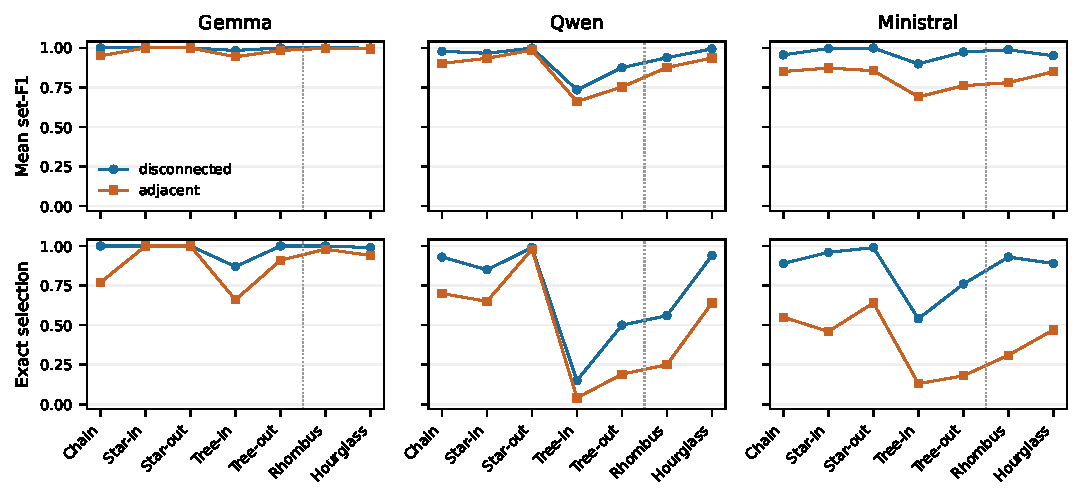
\includegraphics[width=\textwidth]{figures/motif_profiles.pdf}
\caption{Core pattern profiles with source-card triples: disconnected K1 and adjacent K2. Each cell has 100 planned tasks per model/condition; invalid outcomes contribute zero. The first five families have six nodes. Rhombus (four) and hourglass (five), beyond the dotted separator, are not equal-size comparisons. These are descriptive means without inferential error bars. F1 and exact recovery reveal different aspects of failure.}
\Description{Six panels compare F1 and exact selection over seven motifs for three models and two distractor conditions. Incoming trees have low exact recovery, while several outward-star conditions are near ceiling.}
\label{fig:motifs}
\end{figure*}
Figure~\ref{fig:motifs} shows that a single aggregate score conceals large task-family differences. Under K1, six-node star-out exact recovery is 1.00 for Gemma and 0.99 for Qwen and Ministral. Six-node tree-in exact recovery is 0.87, 0.15, and 0.54, respectively. The corresponding tree-in F1 values are 0.984, 0.734, and 0.899. Thus substantial partial overlap can coexist with frequent failure to recover the complete reference. For Qwen, outward-tree exact recovery is 0.50, also below star-out. These comparisons hold node count and candidate-pool size fixed, but not query semantics, relation types, or sampled entities.

The profiles differ across the evaluated models descriptively. Gemma reaches the ceiling for several disconnected families; its remaining difficulty is clearer under exact recovery and adjacent contexts. Qwen's tree-in errors under K1 comprise 83 omission-only outcomes, two mixed outcomes, and 15 exact outcomes out of 100. The failure is predominantly incomplete selection rather than wholesale unrelated selection. We do not infer a hidden search procedure from that observation.

Adjacent contexts expose further differences. Ministral's K2 star-out outcomes include 31 inclusion-only, one mixed, four invalid, and 64 exact outcomes. Its K2 tree-in exact recovery is 0.13, compared with 0.54 in K1. Qwen's tree-in exact recovery falls from 0.15 to 0.04. Gemma's star-out remains at 1.00, whereas its chain exact recovery falls from 1.00 to 0.77. The noise response is therefore not adequately summarized as an identical penalty on every family. These slices are descriptive; we have not tested a model-by-motif-by-noise interaction.

Rhombus and hourglass results complete the evaluated family catalogue but should not determine an equal-size ranking. Their smaller references change the amount of required selection, and their queries differ from several six-node families. In particular, a high hourglass score here does not establish that joins or fan-in are universally easy. We use the family labels to identify empirical task profiles, not to claim a task-independent ordering of abstract graphs.

\subsection{RQ2: Pattern-Specific Size Sensitivity}
\label{sec:rq2}
\begin{figure*}[t]
\centering
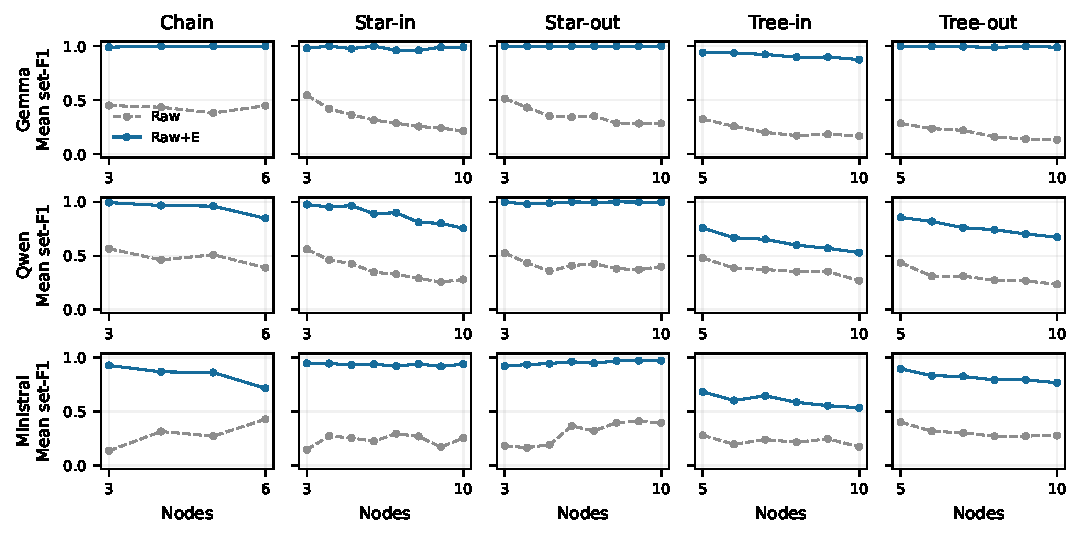
\includegraphics[width=\textwidth]{figures/size_profiles.pdf}
\caption{Size profiles for all variable-size families in Full Raw/Raw+E. Rows are models and columns are families; each point averages 100 planned tasks, retaining invalid outcomes as zero. The pool remains at 25 candidates. Grey dashed lines are Raw; blue solid lines are Raw+E. Sizes are different frozen samples, not paired graph expansions. No inferential error bars or universal monotonicity claim are implied. Rhombus and hourglass have one available size and are omitted from size curves. Appendix~Table~\ref{tab:sizeendpoints} reports endpoint F1 and exact recovery.}
\Description{Fifteen panels show Raw and explicit-overlay F1 against node count for three models and five families. Outgoing stars often remain near ceiling, whereas several chains and trees lose quality.}
\label{fig:sizes}
\end{figure*}
The complete Full Raw/Raw+E grid supports size analysis for all three models, not just Gemma (Figure~\ref{fig:sizes}). However, the observed curves do not support a universal ``more nodes means worse selection'' statement. Under Raw+E, Qwen chain F1 changes from 0.994 at three nodes to 0.848 at six, and Ministral from 0.929 to 0.717. Gemma changes from 0.990 to 1.000. Chain length therefore distinguishes the evaluated models in this condition rather than imposing the same observed degradation on each.

Outward stars provide a contrasting profile. Qwen Raw+E F1 is 0.998 at both three and ten nodes after rounding, while Gemma is 1.000 at both endpoints. Ministral increases from 0.922 to 0.973. These endpoint comparisons do not demonstrate invariance or beneficial causal effects of added nodes: ceiling scores, different accepted samples, and reference prevalence all matter. Inward stars are less stable for Qwen, declining from 0.976 to 0.755 across the same range. Directional family distinctions remain relevant even when both families have a hub-and-leaf description.

Incoming trees deteriorate between five and ten nodes in all three Raw+E model profiles: Gemma F1 changes from 0.940 to 0.875, Qwen from 0.758 to 0.530, and Ministral from 0.685 to 0.536. Exact recovery at these endpoints is 0.67 to 0.60, 0.07 to 0.02, and 0.03 to 0.04, respectively. The latter illustrates why partial and exact metrics must be retained: a lower F1 endpoint does not imply a lower exact endpoint in every small stratum. Some intervening curves are nonmonotonic. Outward-tree endpoint values, and the complete set of size endpoints, are included in Appendix~Table~\ref{tab:sizeendpoints} rather than selecting only decreasing examples.

The size axis simultaneously changes the number of target entities and distractors: reference size $s$ leaves $25-s$ distractors. Even selecting all candidates has F1 $2s/(25+s)$, increasing with $s$. Exact recovery also requires every member of a larger reference to be correct. Consequently, the curves characterize performance on the frozen size grid, not an intrinsic graph-complexity coefficient. The additional Gemma K1/K5 panel is a controlled-format diagnostic; it does not supply a full all-model crossing of size, format, and adjacent noise.

\subsection{RQ3: Evidence Availability and Adjacent Contexts}
\label{sec:rq3}
\begin{table}[t]
\caption{Paired condition effects in score units. Raw contrast: 3,400 pairs/model; noise contrasts: 700. All planned outcomes retained. Bands are exploratory simultaneous bands from the full 78-effect F1/exact family under the fixed-KG/anchor-independence assumptions; they are not new motif/size tests.}
\label{tab:contrasts}
\centering
\small
\begin{tabular}{llrr}
\toprule
Model & Contrast & $\Delta$F1 & Simultaneous band \\
\midrule
Gemma & Raw+E $-$ Raw & +0.674 & [0.664, 0.683] \\
Gemma & Adjacent $-$ disc., triples & -0.016 & [-0.026, -0.007] \\
Gemma & Adjacent $-$ disc., text & -0.023 & [-0.038, -0.008] \\
Qwen & Raw+E $-$ Raw & +0.466 & [0.453, 0.479] \\
Qwen & Adjacent $-$ disc., triples & -0.062 & [-0.086, -0.038] \\
Qwen & Adjacent $-$ disc., text & -0.058 & [-0.082, -0.033] \\
Ministral & Raw+E $-$ Raw & +0.572 & [0.554, 0.590] \\
Ministral & Adjacent $-$ disc., triples & -0.157 & [-0.191, -0.124] \\
Ministral & Adjacent $-$ disc., text & -0.166 & [-0.198, -0.134] \\
\bottomrule
\end{tabular}

\end{table}
Adding explicit relations substantially increases recovery of the graph reference (Table~\ref{tab:contrasts}). Failure-inclusive mean F1 changes from 0.305 to 0.978 for Gemma, 0.386 to 0.852 for Qwen, and 0.275 to 0.847 for Ministral. Paired gains are +0.674, +0.466, and +0.572; all corresponding simultaneous bands are positive under the stated assumptions. The gain remains positive in the both-valid diagnostic, so it is not explained solely by a greater frequency of invalid Raw outcomes. Raw+E adds information rather than merely reformatting an identical fact set. Low Raw agreement cannot be interpreted as a reasoning deficit unless sufficient native evidence is established independently.

In the controlled Core panel, adjacent-minus-disconnected F1 is negative for every model under both triples and templated prose. The six simultaneous bands lie below zero under the conditional bootstrap analysis. Absolute penalties differ substantially, from approximately 0.016--0.023 for Gemma to 0.157--0.166 for Ministral. Context changes include distractor composition and density, so these are not pure causal estimates of an abstract adjacency property. Pattern profiles in Figure~\ref{fig:motifs} show why aggregate penalties should be read alongside family-level failure modes.

The presentation checks are smaller and model-dependent. Qwen's text-minus-triples F1 differences are about $-0.023$ under both question formulations, with negative simultaneous bands; Gemma and Ministral bands include zero. This is not an equivalence finding for those models. Duplicating facts on both cards gives Qwen a +0.041 F1 difference, with simultaneous band [0.024, 0.059], but no uniform benefit across models. Appendix~\ref{app:conditions} reports alternative placement/rendering estimates and all Core condition means, preserving unfavourable and small differences as well as favourable ones.
